\documentclass{acm_proc_article-sp}

\usepackage{algorithm}
\usepackage{algorithmic}

\begin{document}

\title{Addressing Redistribution in Bikeshare Using Cox Processes and Online Supervised Learning}

\numberofauthors{4}
\author{
\alignauthor Walter Dempsey\\
       \affaddr{University of Chicago}\\
       \affaddr{5734 S. University Avenue}\\
       \affaddr{Chicago, IL}\\
       \email{wdempsey@uchicago.edu}
\alignauthor Jette Henderson\\
       \affaddr{The University of Texas at Austin}\\
       \affaddr{Austin, TX 78712}\\
       \email{jette@ices.utexas.edu}
\and
\alignauthor  Vidhur Vohra\\
       \affaddr{Yahoo!}\\
       \affaddr{701 1st Ave}\\
       \affaddr{Sunnyvale, CA}\\
       \email{vvohra@yahoo-inc.com}
\alignauthor  Hunter Owens\\
       \affaddr{University of Chicago}\\
       \affaddr{5734 S. University Avenue}\\
       \affaddr{Chicago, IL}\\
       \email{howens@uchicago.edu}
}


\maketitle

\begin{abstract}
A bicycle sharing system (bikeshare) is a service in which individuals can check-out bicycles from stations for a short period of time and drop them off at any of the stations in the system. The main purpose of bikeshare is to provide transportation for short trips, and it has become common in many cities including New York, Paris, and Beijing. One of the issues with bikeshare is the possible imbalance of bikes across stations, specifically that some stations may have no bikes to check-out while other stations have no slots for arriving bikes. Many cities employ re-distribution techniques on an ad hoc basis. In order to improve the redistribution process, we must estimate the expected number of bikes at a station at some point in the future, as well as the chance that the station becomes empty or full in that time window. To do this, we model the arrival and departure of bikes as a log Gaussian Cox Process. We build a block approximation of the underlying Gaussian processes by clustering  neighborhoods, which will allow for parallel estimation. Moreover, we build online methods for updating the parameters from streaming station data. In order to assess performance, we apply these techniques to the Washington, D.C., bikeshare data. We end with a brief discussion of how our approach can be used in analyzing new stations without sufficient data and as well as new networks/cities. 
\end{abstract}


\terms{Log Gaussian Cox Processes, Block-Approximate Gaussian Processes, Parallel Algorithms, Online Learning}

\section{Introduction}

Bicycle Sharing systems have become ubiqutious over the past several years, providing an alternative mode of transportation and improving the connectivity of their respective cities.  These networks (typically referred to as bikeshare) consist of a number of stations distributed throughout the city with individuals able to check-out bicycles from stations for a short period of time before dropping them off at another station in the system.  A common issue with bikeshare is that traffic patterns commonly result in bike imbalance across stations, with some stations being either empty or full.  We call these {\bf extreme} stations.  These imbalances can lead to delays as bikeshare users must find alternate stations, while also lowering overall ridership due to reliability concerns. Bikeshare systems tackle this issue by some form of redistribution; however, the methods for redistribution of bikes are ad hoc and may be sub-optimal.

For a given time in the future and a station, we aim to predict the number of bikes at the station as well as the probability that the station will become extreme at some point in this time window given its current state as well as auxiliary variables.  This will allow us to predict extreme stations as well as provide an estimated optimal number of bikes that should be at that station to avoid extreme events in the next time window. This foresight will allow bikeshare companies to anticipate extreme stations and keep them from occurring.

We model arrival and departure of bikes at each station as a pair of correlated Poisson Processes.  We propose then modeling the entire bikeshare system as a set of correlated Poisson Processes, where two pairs are correlated based on their spatial proximity.  This set is therefore modeled as a log-Gaussian Cox Process in which we capture station-level, temporal, and spatial random effects.  

This approach is computationally intensive, and therefore we propose approximation methods for estimation, which allow us to run estimation in parallel and provide necessary speedups at the cost of some inexactness.  The bikeshare data analyzed is also streaming, and therefore we provide an online algorithm that updates parameter estimates given the new observations.  This approach allows for updating models given new data without re-fitting the entire model every time.  We end with an application of our techniques to Washington, D.C., bikeshare data.  We analyze the performance of our method and provide methods for prediction of new stations given estimation from surrounding stations.


\section{Arrival and Departure Processes at a Single Station}

We start by considering the temporal process at a given station.  Let $Y_i (t)$ denote the number of bikes at the station at time $t$.  The bike count is an integer-valued process with jumps.  We use $Y(t)$ to define a pair of counting processes that we then model.

The {\bf arrival counting process}, $N_i^{a} (t)$ can be defined as the number of bikes arriving at the station up to time~$t$.  Assuming a finite number of bike arrival times in any interval, we can then define these counting processes as:
\begin{align}
N^{a} (t) &= \sum_{s < t} \left | Y_i (s) - Y_i (s-) \right | {\bf 1} \left[ Y_i (s) - Y_i (s-)  > 0 \right] 
\end{align}
The {\bf departure counting process}, $N_i^{d} (t)$ can be defined likewise for bikes leaving the station.  A consideration is that a station which is empty cannot have departures.  Therefore, $Y_i (t) = 0$ in some interval~$[t, t+\delta]$ implies $N_i^{d} (t+\delta) -N_i^{d} (t) = 0$.   Let $A_{d}$ be the set of all such windows.  Then, we assume the departure counting process to be an inhomogenous Poisson point process on the complement of this set, $\mathbb{R}^{+} - A_{d}$.  We consider the same to be true of the arrival process and the window of all times for which the station is full, $A_{f}$.

For now, we ignore these constraints on the process.  We assume that at a station, the arrival and departure counting processes are correlated.  This implies that we can model the pair as a Cox process where the rate parameters includes a station block effect. That is, $N_i^{a} (t)$ ($N_i^{d} (t)$ respectively) are poisson processes with rate parameter $\lambda_i^{a} (t)$ ($\lambda_i^{d} (t)$ respectively) where
\begin{align}
\log \left( \lambda_i^{a} (t) \right) = \mu^{a}_i(t) + b_i
\end{align}
\noindent where $b_i$ is a random station effect.  The rate parameter for the departure process is defined similarly.

\section{Bikeshare System}

We now consider the complete bikeshare system.  Stations in close geographic proximity provide auxiliary information which should be leveraged.  For example, if a station has many arrivals in a given morning, this is a strong indicator that the number of arrivals at a neighboring station will also be high. Figure~\ref{fig:stations_54_106_ave}  illustrates this behavior of stations that are in close proximity to one another. These two stations are .05 miles apart, and on average, we can see that they have similar behavior.
\begin{figure} [!h]
\caption{Average number of bikes at two Capital Bikeshare stations closely located to one another}
\centering
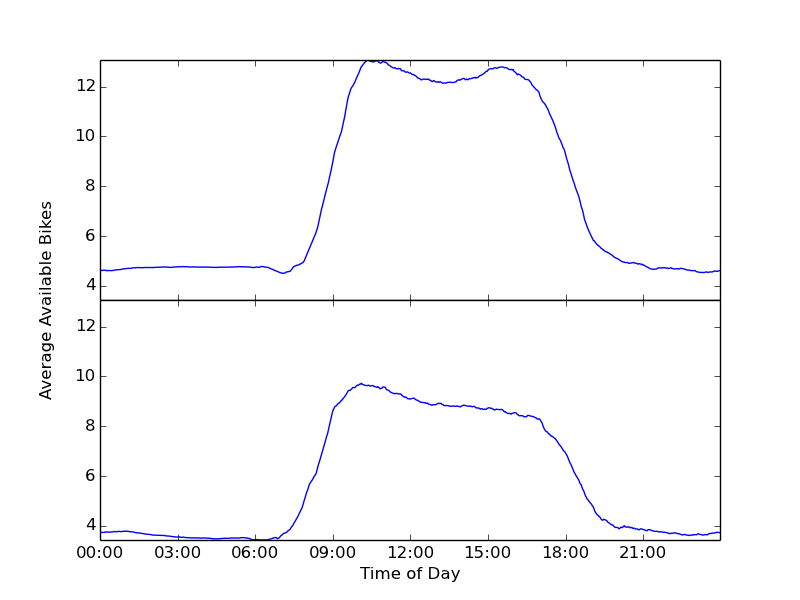
\includegraphics[scale = 0.4]{stations_54_106_ave.png}
\end{figure}
We see the same general trends when looking at a randomly chosen subset of days for one of the stations in Figure~\ref{fig:station_54_6_days}
\begin{figure} [!h]
\caption{Number of bikes at one Capital Bikeshare station over the course of six randomly chosen days}
\centering
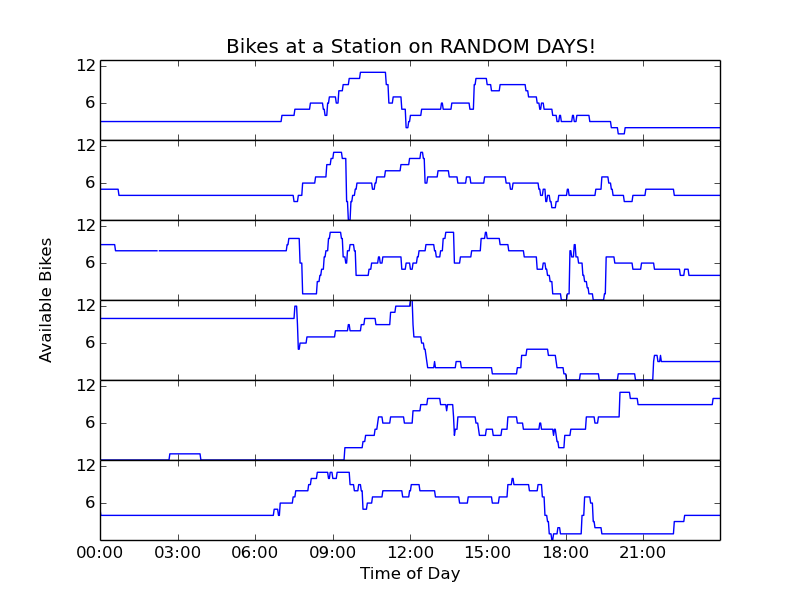
\includegraphics[scale = 0.4]{station_54_6_days.png}
\end{figure}

We wish to introduce the spatial dependency into our current model because of this correlation 

A log-Gaussian Cox Process captures this spatial dependence through random effects in the stochastic rate parameters.  Let $N_i (t) = (N_i^{a} (t), N_i^{d} (t))$ be the pair of counting processes for station~$i$.  Then we can assume that the arrival rate parameters are associated as are the departure rate parameters such that
\begin{align}
\log \left( \lambda_i^{a} (t) \right) = \mu^{a}_i(t) + b_i + Z(t;i)
\end{align}
\noindent where $Z(t;i)$ is a mean-zero gaussian process with covariance that may depend on both time~$t$ and space~$i$.  We can incorporate the station effects into the gaussian process model.  We then consider a simple separable variance components model :
\begin{align*}
\text{cov} ( Z(t;i) , Z(t^\prime; j) ) =& \sigma_0^2 \delta_{t t^\prime}  \delta_{i j} + \sigma_1^2  \delta_{i j} \\
&+ \sigma_2^2 \exp \left( -\frac{ d(i,t),(j,t)) }{\lambda} \right)
\end{align*}
\noindent where $d ( (i,t) , (j,t))$ is a specified distance metric. In our work we consider the $l_1$ distance.  The first term is measurement error at time~$t$ at station~$i$, the second is the random station effect, and the third is a general mean associated with all the arrival parameters.  See Moller et al. \cite{moller:coxproc} for additional details on the Log Gaussian Cox Process.

Covariates can be chosen to account for temporal trends.  We can choose a factor model for $\mu_i^{a} (t)$ that models fixed effects attributable to time of day, month, and year, or a basis expansion in terms of low-order Fourier terms.  In this case, the distance metric will only depend on the location of the stations and the third term will only be included when $t$ and $t^\prime$ are equal.

We assume a similar model for the departure rates.  The random block effects link the arrival and departure processes at a given station, and the third term in the gaussian process links the rate parameters for the arrival processes across stations.  The departure processes across stations are linked via a similar term, albeit different parameter values, $(\sigma_3^2, \lambda^\prime)$.

\section{Maximum Likelihood Estimation}

Fast gaussian process methods for point process intensity estimation have been studied (see Cunningham et al. \cite{cunningham:fastppest}).  We outline a different approach based on combining approximation likelihood with block-approximation of the gaussian process covariance function, and optimization via stochastic gradient descent methods.

Suppose that there are $n$ total stations. Now take the observations at a particular time window, $(t , t+\delta)$ (we model half-hour windows).  The general form of the Cox Process Likelihood associated with the data, \\ $Y(t) = \left( (Y_1^{a} (t), Y_1^{d} (t)), \ldots, (Y_n^{a} (t), Y_n^{d} (t)) \right) $ is:
\begin{align*}
&l_t( \theta; Y(t) ) = \int_{\Lambda} P(Y,  \Lambda | \theta) d \Lambda \\
&= \int\prod_{i=1}^n \frac{\lambda_i^{a} \lambda_i^{d}}{Y_i^{a} Y_i^{d}} \frac{e^{-\lambda_i^{d}-\lambda_i^{a} }}{(2 \pi)^{n} |\Sigma|^{1/2}} \exp \left( (\lambda - \mu (\theta) )^T \Sigma (\theta) ^{-1} (\lambda - \mu (\theta) ) \right) d \lambda \\
&= E_{\lambda | \theta} [l^{\star} ( \lambda; Y(t))]
\end{align*}
\noindent where $l^{\star} ( \lambda; Y)$ is the likelihood for the inhomogeneous Poisson process, and $\lambda$ is the vector of rate parameters for the dual processes at each station.  As we incorporate temporal trends through the the model for the mean, $\mu$, the complete likelihood is the sum over all time windows.  Supposing we have $T$ total time windows, $(t_1, \ldots, t_T)$, then the complete likelihood is:
\begin{align*}
l ( \theta; Y ) = \sum_{i=1}^T  E_{\lambda | \theta} [l^{\star} ( \lambda; Y (t_i)]
\end{align*}
In our setting, the likelihood for each time window consists of estimating an expectation over the finite-dimensional distribution of $\lambda$.  The number of stations is of the order of several hundred.  Washington, D.C. ,has roughly $250$ stations, and therefore the dimension of our expectation is approximately $500$.  The high dimensionality of the integration appears formidable. 

\subsection{Monte Carlo Estimation} \label{mc_estimation}
Standard Monte Carlo methods would employ the estimate:
\begin{equation}
l_{MC} (\theta) = s^{-1} \sum_{j=1}^s l \left( \theta | Y, \lambda^{(j)} \right)
\end{equation}
\noindent where $\lambda^{(j)}$ are simulated realizations of $\lambda$.  This is highly inefficient.  Based on the work of Geyer (1999) \cite{geyer:likinf} and Diggle et al. (2013) \cite{diggle:spatial}, we use the following to provide robust, efficient estimation of the log-likelihood function.  Given un-normalized joint density of $X$ and $\lambda$, $f(X, \lambda | \theta)$, then 
\begin{align}
\hat{L} \left( \theta \right) =& \log \big \{ s^{-1} \sum_{j=1}^s r \left( Y , \lambda^{(j)} , \theta, \theta_0 \right) \big \} \label{approx_lik} \\
&- \log \big \{ s^{-1} \sum_{j=1}^s r \left( X^{(j)} , \lambda^{(j)} , \theta, \theta_0 \right) \big \} \notag
\end{align}
\noindent where $r(X, \lambda, \theta, \theta_0) = f(Y, \lambda | \theta)/f(Y, \lambda | \theta_0)$. The result provides a Monte Carlo approximation to the log-likelihood function, and consequently the maximum likelihood estimate, $\hat{\theta}$, by simulating the process at a single value, $\theta_0$.  The accuracy is a function of the number of simulations, $s$, and the proximity of $\theta_0$ to $\theta$.   Assuming $n$ stations, the density is given by:
\begin{align*}
&\left[ \prod_{i=1}^n \frac{(\lambda_i^a)^{Y_i^a}(\lambda_i^d)^{Y_i^d}}{Y_i^a ! Y_i^d !} e^{-\lambda_i^a - \lambda_i^d} \right] \\
\times& \frac{1}{\sqrt{2 \pi}^n |\Sigma|^{1/2}} \exp \left( (\lambda - \mu(\theta))^T \Sigma(\theta)^{-1} (\lambda - \mu(\theta) ) \right)
\end{align*}
Therefore, the ratio simplifies to:
\begin{align*}
r(Y,\lambda, \theta, \theta_0) =& \left(\frac{|\Sigma (\theta_0)|}{|\Sigma (\theta)|} \right)^{1/2} \\
&\times \frac{\exp \left( (\lambda - \mu(\theta))^T \Sigma(\theta)^{-1} (\lambda - \mu(\theta) ) \right)}{\exp \left( (\lambda - \mu(\theta_0))^T \Sigma(\theta_0)^{-1} (\lambda - \mu(\theta_0) ) \right)} \\
\end{align*}
The pair $(Y^{(j)}, \lambda^{(j)})$ are simulated joint realisations of $X$ and $\lambda$ at $\theta = \theta_0$.  In the first term, $X$ is held fixed and $\lambda^{(j)}$ are conditional on $X$.  Conditional simulation of $\lambda$ requires Markov Chain Monte Carlo (MCMC) methods.  Design, computational issues, and design are detailed by Diggle et al. (2013).  Given a current estimate, $\lambda^\star$, we use a proposal distribution which is a random-walk on the $\log (\lambda^\star)$.
\begin{equation*}
\log (\lambda) \sim N \left( \log \left( \lambda^\star\right) , c \cdot \Xi \right)
\end{equation*}
where $\Xi = - \text{E} \left[ I(\lambda^\star) \right]^{-1}$.  This is given by $\left[ \text{diag} \left( \lambda \right) + \Sigma^{-1} \right]^{-1}$.  The term $c$ controls the acceptance rate for a random walk proposal so that it is tuned to around $0.234$ percent.

Algorithm \ref{applik_alg} outlines pseudocode for finding the maximum likelihood estimate, $\hat{\theta}$.

\begin{algorithm}[!h]
\caption{Approximate Cox Process Estimation} \label{applik_alg}
\begin{algorithmic}
\STATE {\bf ApproxCP}$(Y, s, \theta_0)$
\FOR{$j$ in $1:s$}
\STATE Generate $(\lambda^{(j)}, Y^{(j)})$ at $\theta = \theta_0$
\STATE Generate $\lambda_2^{(j)}$ given $Y$ at $\theta = \theta_0$ via MCMC
\ENDFOR
\STATE Estimate $\hat{L} (\theta)$ by equation~\eqref{approx_lik}
\STATE $\hat{\theta} \gets \arg \max \hat{L} (\theta)$ given $\theta_0$
\end{algorithmic}
\end{algorithm}

It only remains to choose the estimate $\theta_0 = (\mu_0 , {\bf \sigma}_0^2)$.  We estimate the parameters for each Poisson process independently to get initial estimates for the mean parameters, $\mu_0$.  We take the simple average of the estimated mean squared errors for each station, $\bar{\sigma}_i^2 = \left( \bar{\sigma}_{i,a}^2 ,\bar{\sigma}_{i,d}^2 \right)$.  This provides an estimate for $\text{var} (Y)$ across stations.   We use the relationship between the variance of the observed counts, and the variance of the stochastic rate parameters.  Since we have assumed the variance to be stationary, we use the conditional variance formula to show that:
\begin{align*} 
\text{var} \left( Y \right) &= \text{E} \left[ \text{var} \left( Y | \lambda \right) \right] + \text{var} \left( \text{E} \left[ Y | \lambda \right] \right) \\
&= \text{E} \left[ \text{diag} (\lambda) \right] + \text{var} \left( \lambda \right) \\
\end{align*}
\noindent Then we can use the variability of the count data, and subtract the rate parameters from the diagonal to approximate $\text{var}(\lambda)$.  This implies that if we build a semi-variogram, we can use these to estimate $\sigma_1^2$ and $\lambda$.  Moreover, we can estimate the station-level block effects by matching the arrival and departure average mean square errors at the station level and measure the correlation, $\hat{\sigma}_1^2 = \frac{1}{n} \sum_i ( \bar{\sigma}_{i,a}^2  \cdot \bar{\sigma}_{i,a}^2 )^2$.  We can then create the initial estimate for the measurement error by
\begin{equation*}
\sigma_0^2 \approx \frac{1}{n}\sum_i \left[ \sigma^2_{i,a} - \lambda_{i,a} + \sigma^2_{i,d} - \lambda_{i,d}  - 2\cdot \left(\sigma_1^2 - \sigma_2^2 \right) \right]
\end{equation*}

\section{A Parallel Approximate Estimation Algorithm} \label{parallel_estimation}

The assumed dependence among all counting processes makes maximum likelihood estimation computationally intensive.  This is due to the covariance being positive between any two stations.  Therefore, we must model the entire system of counting processes simultaneously and the dimension of the gaussian process becomes prohibitively large.  For example, there are over $100$ loading stations in Chicago for which we have almost a year of data.  If we disaggregate the data to half-hour windows, the complete set of observations is over one-million.  Given the computational cost of the high-dimensional integral, we cannot hope to estimate our model in a practical amount of time.

We start by assuming we capture the temporal dependence through a factor model.  However, we still must worry about the spatial dependence as the dimension would still exceed $10,000$.   However, the dependency, while positive, is weak for stations that are well-separated.  Therefore, we can approximate the true underlying gaussian process by a block-approximate gaussian process, which exploits the weak dependence between stations that are far apart.  Alternative methods exist such as the low-rank covariance matrix approximations (see Chen et al. \cite{chen:lowrank}).  However, Stein \cite{stein:spatial} shows that block-approximation often provides much better approximation to the likelihood than a low rank approximation.

\subsection{Hierarchical Clustering}\label{clustering}
In order to approximate the gaussian process, we must determine the independent station blocks.  This requires partitioning the entire set of stations, $\Omega = \{ {\bf z}_i = (x_i, y_i) \, , i = 1,\ldots S\}$, where $(x_i, y_i)$ are the latitude and longitude for station~$i$. The resulting partition must capture high in-block and low between-block covariance.  

We assumed that the spatial covariance between stations is a decreasing function of the Euclidean distance between the two points.  In particular, we describe the relationship via a squared exponential covariance function, $K(\| {\bf z}_i - {\bf z}_j \|) = \sigma_3^2 \exp \left( - \| {\bf z}_i - {\bf z}_j \|^2/ \lambda \right)$, where $\lambda$ is a range parameter.  This is the limit of the Matern covariance function, a set of stationary covariance functions typically used in spatial statistics.  If we knew the range parameter, $\lambda$, a priori then the partitioning of $\Omega$ can reflect the range of the spatial process.  However, the range is typically unknown before fitting the model, and therefore cannot be used to build the partition.

We therefore perform $k$-means clustering using $l_1$ distance.  The choice of $k$ clusters reflect true neighborhood clustering; moreover, a larger $k$ implies weaker approximations, but faster estimation, while a smaller $k$ implies the opposite.  We therefore choose $k$ to balance the computational-approximation tradeoff.

Figure~\ref{fig:cluster_map} shows the hierarchical clustering applied to the Washington D.C. bikeshare stations.  The clusters reflect the well-defined neighborhoods for the most part. We focus our efforts on the clusters that most closely match well-defined neighborhoods.

\begin{figure} [!h]
\caption{Hierarchical K-means Clustering of Bikeshare Stations in Washington, D.C.}
\centering
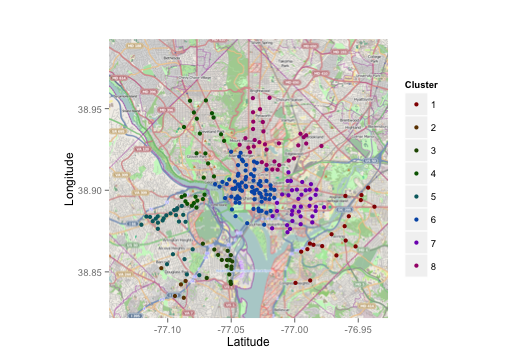
\includegraphics[scale = 0.5]{cluster_map.png}
\label{fig:cluster_map}
\end{figure}

We employ the clustering without knowledge of the range parameter; however, once we have the maximum likelihood estimate, $\hat{\theta}$, we will have an estimate of the range parameter, $\hat{\lambda}$.  The $k$-means clustering algorithm does not consider linear scaling of the distance function.  Therefore, if we simply re-estimate the clusters using the modified Euclidean distance, $\|{\bf z}_i - {\bf z}_j \| / \hat{\lambda}$, we will achieve the same partition.  However, we can now use the range estimate, to choose $k$ more. 

\subsection{Parallel Estimation}

The block-diagonal approximation lightens the computational burden of the Monte-Carlo Simulations, as the conditional simulation of $\lambda$ condtional on $Y$ can be done in parallel.  However, the likelihood does not factorize by cluster under the current assumptions.  The approximate likelihood, $\hat{L} (\theta)$, does become a sum over independent clusters, but the assumption of common variance components means that estimation cannot be done in parallel across clusters.

If we assume that the variance components are distinct for each cluster, then we can estimate parameters separately for each cluster by exploiting variational independence.  This leads to additional computational savings as we can then parallelize the entire estimation procedure.  If the true variance components are identical for each cluster, then the estimated variance components for each cluster will be unbiased estimators.  Therefore, we only sacrifice slight losses in efficiency for gross gains in speed.  

\begin{algorithm}[!h]
\caption{Approximate Likelihood Algorithm} \label{applik_alg}
\begin{algorithmic}
\FOR{$i$ in stations}
\STATE $\mu_i \gets$ Fit marginal model $i$ 
\ENDFOR
\STATE Obtain initial estimate for $\sigma_0^2 = \text{mean} \{ \sigma_{0,j}^2\}$
\STATE Obtain initial estimate for $\sigma_1^2 = \sigma_2^2 = \sigma_0^2 / 2$
\STATE $U_1, U_2, \ldots U_k \gets$ cluster$(k, \text{stations})$
\FOR{$j$ in $1:k$}
\STATE $\theta_j \gets \text{ApproxCP} (Y_j, s, \theta_0)$ for Cluster $U_j$
\ENDFOR
\end{algorithmic}
\end{algorithm}

Given the approximate maximum likelihood estimate, $\theta$, we now turn our attention to estimating the desired quantities.

\section{Prediction}

For a particular station~$i$ at a particular time~$t$, we know the number of bikes at the station, $Y_i(t)$.  We are interested in estimation of the expected number of bikes at some future time point, $t+\delta$.  To answer the question of re-distribution, we also need to know the probability that the number of bikes reaches an extreme value in the time window $(t, t+\delta)$.  Therefore, assuming a maximum number of spots $\tau$, we want to estimate $\text{E} \left[ Y(t+ \delta) | Y(t) , \hat{\theta} \right]$ and 
\begin{equation*}
\text{P} [ Y(s) = 0 \text{ or } Y(s) = \tau \text{ for some } s \in (t, t+\delta) | Y(t), \hat{\theta} ].  
\end{equation*}

\subsection{Expected Number of Bikes}
Our block approximation from section~\ref{parallel_estimation} allows estimation of both quantities to be done separately for each cluster.  Suppose station~$i$ sits inside cluster $U \subset \Omega$.  Let the expected rate parameter at time~$s$ given $(Y,\hat{\theta})$ to be given by~$\hat{\lambda} (s)$.  Then the expected number of arrivals in the window is given by $\int_{t}^{t+\delta} \hat{\lambda}_a (s) ds$.  The expected number of departures is the same formula with the integrand replaced by $\hat{\lambda}_d$.  Then we can estimate the expected number of bikes at the station by:
\begin{equation*}
\text{E}_{\hat{\theta}} \left[ Y(t+ \delta) \, | \, Y(t) \right] = Y(t) + \int_{t}^{t+\delta} \hat{\lambda}_a (s) ds - \int_{t}^{t+\delta} \hat{\lambda}_d (s) ds
\end{equation*}

To calculate the expected rate parameter at time~$s$, we need to calculate the probability of the rate parameter given the maximum likelihood estimate and the observed counts. The predicted rate parameter is given by:
\begin{equation*}
P [ \lambda_i (s) | Y, \hat{\theta} ] \propto \int P [ Y | \lambda (s), \hat{\theta} ] P [ \lambda_i (s) | \hat{\theta} ] \prod_{j \neq i} P [ \lambda_j (s) | \hat{\theta} ] d \lambda_j (s)
\end{equation*}
\noindent We assume that the rate parameter is constant in each half-hour time window.  Let $N^{a}_i(t, t+\delta)$ be the number of arrivals in the time window starting at time~$t$ at station~$i$.  Then let $N^{a} (t, t+\delta)$ be the vector of arrivals for stations in cluster $U$.  Then we can estimate the rate parameter for window $(t, t+\delta)$, $\lambda$ by 
\begin{equation*}
\int_0^\infty \lambda P [ \lambda | N^{a}, \hat{\theta} ] d\lambda
\end{equation*}
\noindent We calculate these expectations by Monte Carlo estimation.  The expected number of bikes is then a simple difference of the Monte Carlo estimated expected arrival and departure rate parameters added to the total number of current bikes.  Because the intervals are independent, the expected number of bikes in the future is just the sum of independently estimated rate parameters for each disjoint window.

\subsection{Probability of Station Being Extreme}

To calculate the probability of station~$j$ being empty in the time window (denoted $P_j (t, t+\delta)$) requires a simulation-based approach.  Suppose we are interested in the probability over the smallest window, $(t, t+\delta)$.  We start by generating the constant arrival and departure rate parameters in the window for station~$j$ in $U$, $\lambda^{a}_j$ and $\lambda^{d}_j$ respectively. 

Then for a particular station, we can wish to simulate the arrivals and departure of bikes.  Given the rate parameters, the arrival and departure processes are independent, and, therefore, the superposition principle implies that the first event has an exponential waiting time, $T_1$, with rate parameter $\lambda_j = \lambda^{a}_j + \lambda^{d}_j$.  The probability that the first event is an arrival is $\lambda^{a}_j / \lambda_j$.   If $T_1 < \delta$, then we have an event in the time window.  If that event was an arrival, then we set $Y(t+T_1) = Y(t) + 1$.  If the event was a departure, then we subtract one from the current number.  We then continue this process until $\sum_{k} T_k > \delta$.  We then have a random instance of $\{ Y_j(s) \, s \in (t, t+\delta) | Y_j(t) \}$.  We do this for each station~$j$ in $U$.

The number of bikes is bounded to be in $[0, \tau_j]$, where $\tau_j$ is the maximum number of slots at station~$j$.  Therefore, if the number of bikes is zero in the time window, we cannot generate a departure.  The same is true for a full station and generating arrivals.  We can handle these constraints in two ways.  We can continue to generate these departures and arrivals but ignore those that push the process outside of its boundaries.  By the thinning principle, this is equivalent to only generating arrivals at the rate $\lambda^{a}_j$ when the station is empty or departures at the rate $\lambda^{d}_j$ when the station is full.   On the other hand, instead of ignoring the arrivals, we can send these arrivals to nearby stations.  This will be more accurate; however, we would then need to estimate the travel time to the nearest station that is not full.  We do not currently employ such methods, as they add a serious additional computational obstacle.  However, our current framework is highly adaptable, and we could incorporate this approach.

Let $\Delta^{(i)}_j$ be an indicator that the number of bikes at station $j$ reaches an extreme position in the time window for the~$i$th instance from our simulation.  Then we estimate the probability by the simple average:
\begin{equation*}
\hat{P}_j = \bar{\Delta}_j = s^{-1} \sum_{i=1}^s \Delta^{(i)}_j
\end{equation*}
\noindent  These are simultaneously estimated for each station in the cluster.  We can therefore estimate the probabilities in parallel for each cluster, $U_1$ through $U_k$.

\subsection{Proper Distribution of Bikes}

The above provides detailed information that will allow bikeshare companies to redistribute bikes  proactively before stations become empty.  We now answer the question of appropriate distribution of bikes.  That is, before commuting hours, what is the correct distribution of bikes across stations in a city that will minimize the chance of a station becoming extreme? 

Let $Y$ be a vector containing the number of bikes at each station in the city.  Then we can calculate the probabilty of each stations becoming extreme in the desired time window, $P$.  For example, we may be interested in the time window that lasts from one hour before rush hour to several hours after rush hour ($6$AM to $12$PM for instance).  We then assume some objective function of the probabilities, $f: P \rightarrow \mathbb{R}$.  For example, we may be interested in minimizing the maximum, $f(P) = \max_j P_j$, or in miniming the sum of squares, $f(P) = \sum_j P_j^2$.  

The goal is then to find the best allocation of bikes for the city with the constraint on the total number of bikes in the system remaining fixed, $\| Y\|_1 = C$.  In particular,
\begin{align*}
&\max f (P) \\
\text{s.t. } P = \{ P[ Y_j(s) &\text{ extreme for } s \in (t,t+\delta) | Y_j (t) \} \\
&\text{and } \| Y \|_1 = C
\end{align*}
We can add additional constraints that may be necessary in practice.  For example, we may require a certain number of bikes per neighborhood.  The search space is quite large.  Given $C$ total bikes and $N$ total stations, the search space is of size $N^C$.  Therefore, given $f$ and $Y$, we propose a simple simulated annealing approach to finding the global optimum.  Details are given by Bertsimas and Tsitsikis (Statistical Science).

The annealing approach requires an initial state.  We assume that the system currently is working at least approximately close to an optimum.  Therefore, we take $Y_0$ to be approximately the average number of bikes at each station at time $t$.  Simulated annealing produces $\hat{Y}$.  As we only care about distribution at a few distinct times, we only need to calculate optimum allocation several times. 

Slight changes to the objective function may result in drastically different distributions of bikes across the city.  It is necessary to investigate this behavior.  For example, we can have the objective function take into account the rate parameters, penalizing empty, busy stations more than empty, idle ones.  This does not increase the search space as the rate parameters are not functions of $Y$; however, it does add additional computational burdens. 

The optimum allocation minimizes the re-distribution thoughout the day, saving resources and time.


\section{Estimation and Prediction for a New Station} \label{newstation}

Many bicyle sharing systems grow over time.  In Chicago, over $50$ new stations have been added in the past few months.  Even in cities with long-standing bikeshare systems, new stations are added as citizens of neighborhoods continue to request additional capacity.  It is therefore necessary to be able to estimate parameters for new stations even before we have much data on the new station.

Let $z=(x,y)$ denote the latitude and longitude of the new station.  Then we calculate the distance from the new station to the centroids of the various clusters discussed in Section~\ref{clustering}.  We then assume that the new station will be added to the cluster such that the centroid of the cluster is closest in Euclidean distance.

Within this cluster, we calculate a weighted average of the parameters at each station, $\theta_j$, where the weights are proportional to the exponential squared covariance function.  We use this as an initial estimate 
\begin{equation}
\hat{\theta} = \frac{\sum_j \exp \left( - \frac{ |z - z_j|}{\lambda} \right) \theta_j}{\sum_j \exp \left( - \frac{ |z - z_j|}{\lambda} \right) }
\end{equation}
\noindent where the sum is over all stations in the assigned cluster.  Prediction then occurs in the same manner, where we employ Kriging methods for interpolation of the spatial process to the new station location.

We may have a point on or near the boundary.  In that case, we can then assign the new station to each cluster with probability proportional to the exponential squared distance from the centroids.  Then the above estimate is denoted $\hat{\theta}_i$ for cluster $U_i$ and the estimated parameters become the weighted average of the above estimates.  The predictions are handles in a similar way, and prediction for each cluster is done separately and then compiled by weighted averaging.

Once we have collected enough data for the station, we can then revert to standard estimation procedures.  Section~\ref{online_learning}  outlines a different approach to the above, and provides additional tools for estimation of parameters given new data is continually streaming.

\section{Online Learning: Algorithm and Prediction} \label{online_learning}

Unlike other spatial-temporal datasets, the bikeshare datasets are continually updated each day.  Each day generates an observation of the underlying stochastic process. Unfortunately, the methods outlined above are computationally expensive and too slow to be re-fit on a daily basis.  Moreover, if we assume that the system is in equilibrium (meaning parameter values are constant and not changing) then once we have enough data, the additional observations will only be marginally useful and continuing to fit the model will be unnecessary.

However, the bikeshare systems do change over time as does their use.  Moreover, for new stations, we'd like a more natural manner for switching from the weighted average to estimation of the .  We provide such an approach below.

Our assumption that the temporal trends are captured in the mean model implied that the stochastic process over disjoint time windows is independent.  The likelihood then factorized into a sum over these disjoint time windows.  When the likelihood factorizes into the sum of differentiable functions, stochastic gradient descent methods can be used for finding the maximum likelihood estimate (see Bottou \cite{bottou:sgd} for further details of stochastic gradient descent in large-scale machine learning).

In stochastic gradient descent, the true gradient of the function $\frac{\partial}{\partial \theta} L( \theta)$ is approximated by the gradient at a single time window, $(t, t+\delta)$.  Updates are then given by:
\begin{equation}
\theta_{t+1} \gets \theta_{t} + \gamma_t \nabla L_t (\theta) 
\end{equation}
\noindent where $\gamma_t$ is the step size, and $L_t$ is the likelihood given the observations at time $t$.  Also, $\theta_t$ is the estimate of the parameter by employing SGD using data in sequence up to time~$t$.  We start with the same initial estimates as described in Algorithm~\ref{applik_alg}.  We hope that this algorithm behaves like its expectation, despite the noise introduced by using only one time window at each step.  We cycle through the time windows until convergence is reached. Convergence results typically require the step size to be a decreasing sequence 
\begin{equation} \label{sgd_conditions}
\sum_{t} \epsilon_t^2 < \infty \hspace{0.2 cm} \text{and} \hspace{0.2cm} \sum_{t} \epsilon_t = \infty
\end{equation}
\noindent We start with the first time window and work forward, shrinking the step size as a rate of $O(n^{\alpha})$ for $\alpha < \frac{1}{2}$ to ensure convergence.  We approximate the derivative of the likelihood based on the Monte Carlo approach outlined in Section~\ref{mc_estimation}.  Given the current estimate, $\hat{\theta}$ we can then update the parameters for each day of data without having to refit the entire model.

This requires calculating the derivative of the likelihood.  We instead calculate the derivative of the approximate log-likelihood.
\begin{align*}
\frac{\partial}{\partial \theta} \hat{L} \left( \theta) \right) =& \frac{\sum_{j=1}^s \frac{\partial}{\partial \theta} r \left( Y , \lambda^{(j)} , \theta, \theta_0 \right) }{\sum_{j=1}^s r \left( Y , \lambda^{(j)} , \theta, \theta_0 \right) } \\
&-\frac{\sum_{j=1}^s \frac{\partial}{\partial \theta} r \left( Y^{(j)} , \lambda^{(j)} , \theta, \theta_0 \right) }{\sum_{j=1}^s r \left( Y^{(j)} , \lambda^{(j)} , \theta, \theta_0 \right) }
\end{align*}
So it rests to find the derivative with respect to $\theta$ of $r(Y,\lambda, \theta, \theta_0)$.  We assume that the we have a linear mean model, $\mu(\theta) = X \beta$ and a variance components model, $\Sigma = \sum_k \sigma_k^2 K_k$.  Then taking the derivative with respect to $\beta$ and $\sigma_j^2$:
\begin{align*}
\frac{\partial}{\partial \beta} r(X,\lambda, \theta, \theta_0) =& \frac{X^T \Sigma^{-1} \left( \lambda  - X \beta \right) }{\exp \left( (\lambda - \mu(\theta_0))^T \Sigma(\theta_0)^{-1} (\lambda - \mu(\theta_0) ) \right)} \\
\frac{\partial}{\partial \sigma^2_j} r(X,\lambda, \theta, \theta_0) =& \frac{(\lambda - X \beta)^T \Sigma^{-1} K_j \Sigma^{-1} \left( \lambda  - X \beta \right) }{\exp \left( (\lambda - \mu(\theta_0))^T \Sigma(\theta_0)^{-1} (\lambda - \mu(\theta_0) ) \right)} \\
\end{align*}
The numerator in both cases is the typical derivative one would see for normal distributions.  The denominator is constant, and it implies we can further simplify the derivative of the approximate likelihood:
\begin{align*}
\frac{\partial}{\partial \beta} \hat{L} \left( \theta) \right) =& \frac{\sum_{j=1}^s X^T \Sigma^{-1} \left( \lambda^{(j)}  - X \beta \right) }{\sum_{j=1}^s  \exp \left( (\lambda^{(j)} - X\beta)^T \Sigma^{-1} (\lambda^{(j)} - X\beta) \right)} \\
&- \frac{\sum_{j=1}^s X^T \Sigma^{-1} \left( \lambda^{(j)}  - X \beta \right) }{\sum_{j=1}^s  \exp \left( (\lambda^{(j)} - X\beta)^T \Sigma^{-1} (\lambda^{(j)} - X\beta) \right)} \\
\frac{\partial}{\partial \sigma^2_j} \hat{L} \left( \theta) \right) =& \frac{\sum_{j=1}^s (\lambda^{(j)} - X\beta)^T \Sigma^{-1} K_j \Sigma^{-1} \left( \lambda^{(j)}  - X \beta \right) }{\sum_{j=1}^s  \exp \left( (\lambda^{(j)} - X\beta)^T \Sigma^{-1} (\lambda^{(j)} - X\beta) \right)} \\
&- \frac{\sum_{j=1}^s (\lambda^{(j)} - X\beta)^T \Sigma^{-1} K_j \Sigma^{-1} \left( \lambda^{(j)}  - X \beta \right) }{\sum_{j=1}^s  \exp \left( (\lambda^{(j)} - X\beta)^T \Sigma^{-1} (\lambda^{(j)} - X\beta) \right)} \\
\end{align*}
again where the first term has the $\lambda^{(j)}$ from simulations of the joint distribution given $\theta = \theta_0$ and the latter term has the $\lambda^{(j)}$ from simulations given the data, $Y$, and $\theta = \theta_0$.

In Section~\ref{newstation} we introduced the estimation procedure for parameters associated with a new station.  The stochastic gradient descent algorithm provides a natural mechanism for moving from this initial estimate toward the true Moreover,introduction of a new station may change the rate parameters associated with the neighboring stations.  In that sense, SGD is a consistent and straightforward approach when we wish to .  When we introduce a new station, the step size is increased in order to reflect the potential changes to the parameters.  However, if there are no further changes to the system, the step size decreases again in the same manner such that conditions~\eqref{sgd_conditions} are met.



\section{Experimental Results}

\vspace{0.25cm}

\subsection{Washington D.C. Bikeshare}
\vspace{0.25cm}
{\bf SECTION OUTLINE}

We will test our method using data from the Washington, D.C. bikeshare system. This data set consists of station-level reports of the number of bikes and empty slots every minute. We augmented this data with weather data recorded on an hourly basis.

In addition to the station-level data, we also use data that deals with the redistribution of bicycles by bikeshare employees. Each time a bike share driver employees up or drops off bikes at a station, the bikeshare company records the trip. We refer to this redistribution of bicycles as rebalancing. Capital Bikeshare, the bikeshare system in Washington , D.C.,  provided us with rebalancing data covering a year of rebalancing trips. This data contains the starting and ending stations for a bicycle and the times the bicycle was picked up and dropped off at another station. We used this data to remove rebalancing events from the station-level data. Specifically, if a rebalancing event occurred during a timeframe of interest, we subtracted the number of bikes arriving to the station via rebalancing from the total number of bikes that arrived during the timeframe.

In our analysis of the Washington, D.C., bikeshare data, a few patterns emerged around high activity times. The figure below anecdotally illustrates these common usage patterns. The purple line is the average number of bicycles at a bikeshare station located in downtown D.C., and the green line is the average number of bicycles at a bikeshare station located in an area of D.C. that is more residential. The averages were taken for every Monday over a year-long period. In the morning, the residential station empties out as people head to work and the downtown station fills up as people arrive at work. This figure demonstrates two potential problems in a bikeshare system, specifically riders can arrive at bike stations to check-in a bike but find no slots to dock their bike or potential riders arrive at a station to check out bikes but there are no bikes available.  For this predictive model to be useful, it must perform well during these ``high activity'' times at the stations. Specifically our goal is to mitigate these situations in high activity times.

\begin{figure} [!h]
\caption{Average number of bikes at two Capital Bikeshare Stations taken over every Monday in one year}
\centering
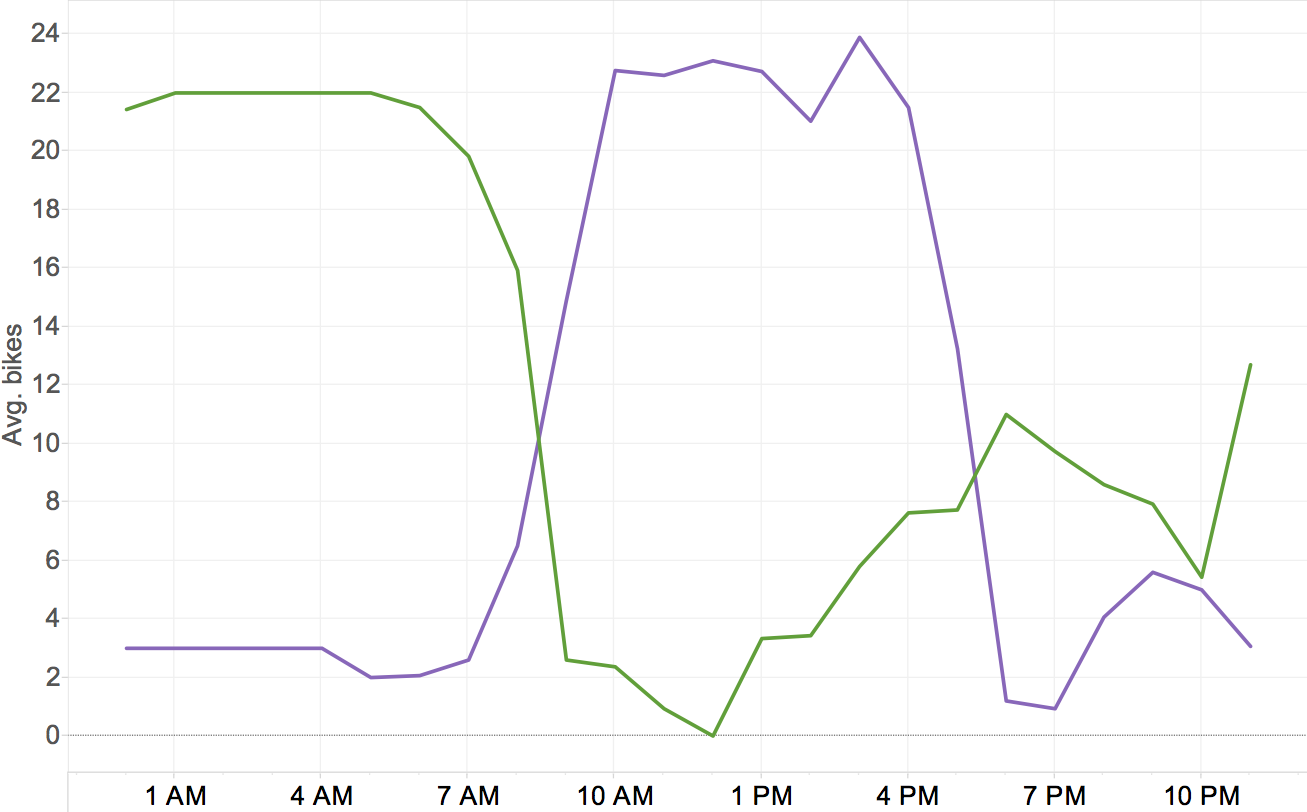
\includegraphics[scale = 0.35]{stations_over_time.png}
\end{figure}

Different usage patterns may manifest in other bikeshare systems. For example, a drastic elevation change in a city could lead to riders using bikeshare on the way downhill but other public transit options on the way uphill (see \cite{lin:chou}).
\vspace{0.5cm}

\subsection{Performance Indices}

We wish to measure the success of our current modeling approach.  We were interested in estimating two specific quantities for a given station: (1) the expected number of bikes at some point in the future given the current number of bikes, $E_{j, \theta} (t+\delta | t) = E[ Y_j(t+\delta) | Y_j(t), \theta]$, and (2) the probability of the station becoming extreme during this time window, $P_{j,\theta} (t, t+\delta)$.

For station~$j$, at time~$t$ with window length $\delta$, we use the mean-squared error of prediction in both cases to measure success of the algorithm:
\begin{align}
F_1(j, t, \delta) = \sum_{t^\prime = t} \| Y_j(t + \delta) - E_{j,\hat{\theta}} [ t+\delta | t] \| \\
F_2(j, t, \delta) = \sum_{t^\prime = t} \| \Delta_j(t,t + \delta) - P_{j,\hat{\theta}} ( t, t+\delta) \|
\end{align}

\vspace{0.25cm}
%{\bf SECTION OUTLINE}
%\begin{enumerate}
%\item How do we measure success?
Using the rate parameters estimated by the Poisson model and the current number of bikes at a station, we can simulate bike availability in the future. For example, in the distributions below, the pink distribution was generated by setting the number of initial bikes at 16 and simulating what happens to the station over the next two hours - thousands of times. The blue distribution is the result of thousands of simulations initialized at 22 bikes.

\begin{figure} [!h]
\caption{Distribution of bikes at a station given different initial number of bikes at a start time}
\centering
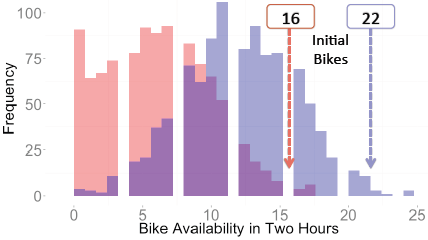
\includegraphics[scale = 0.5]{poisson_simulated_number_of_bikes.png}
\end{figure}
Not unexpectedly, simulating with fewer bikes increases the likelihood that the station will be empty at the end of the two hours. Wether the station had 16 or 22 bikes at 9AM, our model tells us that bikes tend to leave this station over the next two hours, which is why our station simulations so infrequently end up with the same number of bikes they start with.


So we can use simulation to infer conditional distributions - given an initial number of bikes at this time of the day, what is the distribution of the number of bikes we'll end up with after two hours? But we can also, given any initial value of bikes, calculate the probability of a bike station emptying out or filling at any point during the time interval. Then, for any tolerance level - I want the station to be empty during the next two hours less than one in five times - we can suggest the appropriate number of bikes to put at the station. The graph below demonstrates this idea.

\begin{figure} [!h]
\caption{Distribution of bikes at a station given different initial number of bikes at a start time}
\centering
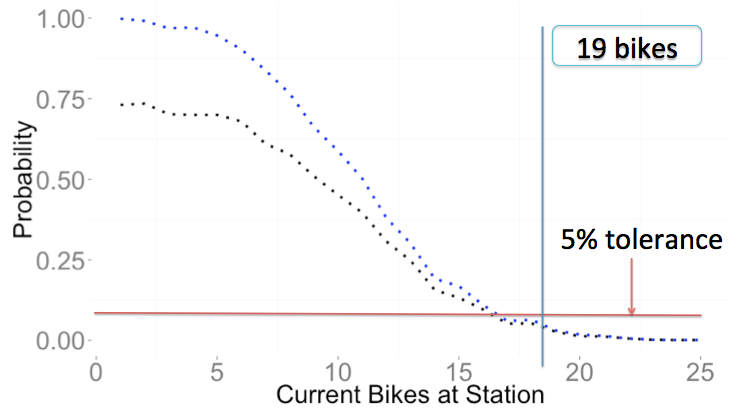
\includegraphics[scale = 0.3]{pr_of_empty_station.png}
\end{figure}

The x-axis is the number of bikes at a station at beginning of the time interval - 7 AM, in this case. The y-axis is the probability that the station will be empty.

The blue line is the probability that the station will be empty at any time between 7 AM and 9 AM, as a function of the number of bikes initially at the station. For example, if the station has 10 bikes at 7 AM, the probability that the station will be empty at some point between 7 AM and 9 AM is about 60\%.

The black line is the probability that the station will be empty right at 9 AM. Using the same example as before, if the station starts with 10 bikes, the probability that it will be empty at 9 AM is about 50\%.

Now we can pick a tolerance level and figure out how many bikes we need to put at the station to achieve this tolerance level. Say that we want to be 95\% sure (or have a tolerance of 5\%) that the station does not empty out in the next two hours. This plot shows us that we need to initially stock the station with 19 bikes to be 95\% sure.


%\item We need good short term (`15 min' predictions) vs long term predictions of counts
%\item We also want good prediction of the probability of being empty or full?
%\item Need baseline and alternatives for comparison
%\end{enumerate}
\vspace{0.5cm}

\section{Summary}
Moving people around efficiently in cities a fundamental problem in urban planning as city populations continue to grow. Bikeshare widens the transportation options for a city's citizens. Bikeshare also has the capacity to make other public transportation options more feasible by connecting people to bus stops and train stations that are too far to get to on foot. It is a creative approach to a modern transportation problem, and using predictive modeling, we show a method to ensure bikeshare companies have a proactive tool to deal with extreme stations. Currently, we model bike arrivals and departures at a given station and show how correlation with other stations can be incorporated to gain a better understanding of the state of the bikeshare system. 

\bibliographystyle{plain}
\bibliography{bibliography}

\end{document}
